\section{Workload Analysis}

%In the emerging cloud computing world, users are able to process larger amount of data because tools such like Hadoop are available. 
The workload of a scalable file system is determined
by its user workloads and the structure of the tools they use.
To guide the design of scalable metadata service,
we will first analyze the workloads seen by related file systems.
We will collect both static and dynamic metadata samples.
Static metadata includes file size distribution,
file counts in directories, and path depth which shows the statistics of the file system at rest.
This has been reported often, even for HPC systems\cite{dayal2008storage, welch13}.
These stats could affect the cost of various operations.
For example, deeper directories require more lookups for pathname resolution.
But more importantly, and  much more rarely reported,
dynamic metadata is the workloads applied to the system,
e.g. percentage of different operations, locality in the pathnames and etc.
We may further disaggregate these operations by important use case classes like MapReduce and table stores.

Existing data about workload analysis is mainly about smaller and older systems at rest. 
Dynamic workload analysis relies on more expensive trace capture. 


Two studies on dynamic network file system workloads \cite{leung2008measurement,anderson2009capture}
show that most metadata operations are related to $open$, $getattr$ and $directory read$.
File systems study shows similar trends in HP-UX and Windows NT systems\cite{roselli2000comparison}.
These studies  focus on data access patterns much more than on metadata.
One of the most extensive static workload is
five-year study from campus workstations in Microsoft \cite{agrawal2007five}.
The newest large system static analysis data is presented in Welch's paper \cite{welch13} 
on  65 HPC customer  clusters. 
They show that though most capacity is still occupied by large files,
most files are still small,  which is similar to the observation in \cite{dayal2008storage}.
The large number of small files potentially increase
ratio between metadata operations and data operations.
Because DISC and cloud workloads are different from HPC workloads,  we want to know if the file systems workloads are different too.

%As shown in Figure~\ref{fig:capacity_size}, most capacity is used by large files. However, Figure~\ref{fig:filenum_size} shows that  $70\%$ to $90\%$ files in these various systems are smaller than 64MB.

\begin{table}[tH]
  \centering
  \begin{tabular}[th]{|c|c|c|c|c|c|}
    \multicolumn{6}{c}{File Size Distribution}\\ 
    \hline
    ID & Description & \# of Nodes & Raw Capacity & \# of Files &
    Avg. File Size \\
    \hline
    \hline
    DW & unknown & 2000 & 21 PB & 40.0 M & 67.04 MB\\
    OC & Research& 64 & 0.3 PB & 5.7 M & 8.21 MB\\
    M45 & Research& 400 & 1.5 PB & 21.8 M & 23.62 MB\\
    A & Sandbox& 1800 & 3.8 PB & 41.8 M & 28.14 MB\\
    C & Research& 800 & 3.5 PB & 10.1 M & 41.03 MB\\
    D & Production& 3000 & 6.5 PB & 23.4 M & 102.09 MB\\
    M & Research& 2000 & 6.3 PB & 25.5 M & 77.83 MB\\
    N & Research& 3500 & 10.6 PB & 35.4 M & 111.41 MB\\
    U & Production& 1700 & 13.0 PB & 17.7 M & 95.30 MB\\
    \hline
  \end{tabular}
  \caption{Clusters from which we collect file size distributions. 
    DW (Data Warehouse) is at Facebook, OC (our cluster), and
    all other clusters are at Yahoo!. DW is  the largest capacity HDFS
  cluster we know about  as of May
  2010~\cite{facebook-datawarehouse}.}
  \label{tab:clusters}
\end{table}


\begin{figure*}[t!h]
    \center
    \subfigure[Fraction of files $\leq x$ bytes]{
        \label{fig:filedistr:file}
        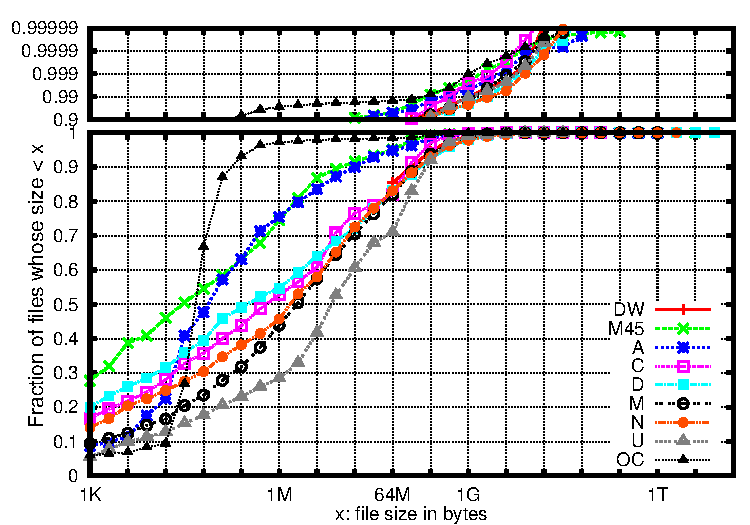
\includegraphics[width=0.4\textwidth]{figs/filenum_CDF}
    }
    \subfigure[Fraction of storage used by files $\leq x$ bytes] {
        \label{fig:filedistr:byte}
        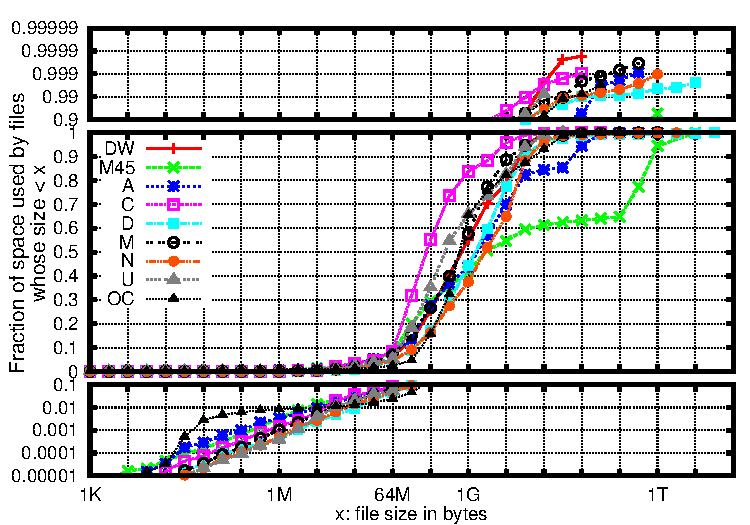
\includegraphics[width=0.4\textwidth]{figs/filesize_CDF}
    }
    \caption{File size distribution} 
    \label{fig:filedistr}
\end{figure*}


We gathered file size  data
from our OpenCloud HDFS cluster and clusters at Facebook and Yahoo! (summarized in
Table~\ref{tab:clusters}).
Figure~\ref{fig:filedistr:file} plots the cumulative distribution function
(CDF) of file size.  Across all clusters, the largest single file
observed is about 2.7~TB; the median size ranges widely from 16~KB to 6~MB, and the average 
ranges from 8~MB to 108~MB. 
Compared with HPC file systems reported by Dayal et al \cite{Dayal08} where
 median file size ranges from 2~KB to 256~KB and mean from 169~KB to 29~MB,
file systems for cloud computing  have  considerably bigger files. 
Yet even with these ``large'' files, at least $70\%$ and as many as $99\%$ of
files are smaller than 64MB (1 HDFS block), as shown in Figure~\ref{fig:filedistr:file}.
Figure~\ref{fig:filedistr:byte} plots the CDF of space used by files up to a
particular size. 
Across all clusters 40\% to 80\% of the storage capacity
is consumed by files smaller than 1GB (16 blocks);
in cluster C, at the extreme,  55\% of  capacity is used by files smaller than
256~MB (4 blocks). Facebook's DW cluster, the largest, has some 2PB of files
smaller than 256MB. 



We believe that many large clusters running parallel jobs may exhibit ``weak scaling" for metadata workloads. By this we believe that large jobs on large clusters will increase the frequency of file metadata operations much more than directory metadata operations. We seek evidence for the assertion and distribution parameters, or traces, to drive our evaluation of scalable metadata services.
As shown in \cite{shafeeq2010}, we can use a slow but easy implementation for rename when these operations are rare. The OpenCloud cluster\cite{opencloud} in CMU is composed of compute nodes, (external) IO/storage nodes and login/master nodes. There are  64 compute nodes each with 8 cores, 16GB  DRAM, 4 1TB disks and 10GbE connectivity between nodes. The cluster runs Hadoop 0.20.1. 
Users generally log into login node and submit Hadoop jobs.
In the OpenCloud cluster, we see that most operations are simple file operations like open(). It's easier for a system to scale simple operations. 
We also want to learn whether there are characteristic patterns by applications that the system could optimize for. For example, we know that for Hadoop jobs, the file names are generated by specific patterns. For each task, a temporary directory is created under the output directory. Output files from the task are stored in the temporary directory first and  will be renamed to the output directory when the task succeeds. The temporary directory will be deleted after rename. 
We could replace the temporary directory by adding a prefix to file names to avoid creating and deleting the temporary directories. Another optimization might be process the files of a  directory by one server after recognizing a less busy pattern. 
If there are  only a few files generated by each map or reduce task, there's less need to use multiple servers for such a small directory, at least until the number of cores in a cluster exceeds tens of thousands.

\begin{figure*}[t!h]
    \center
    \subfigure[Operation count]{
      \label{fig:opstats:count}
      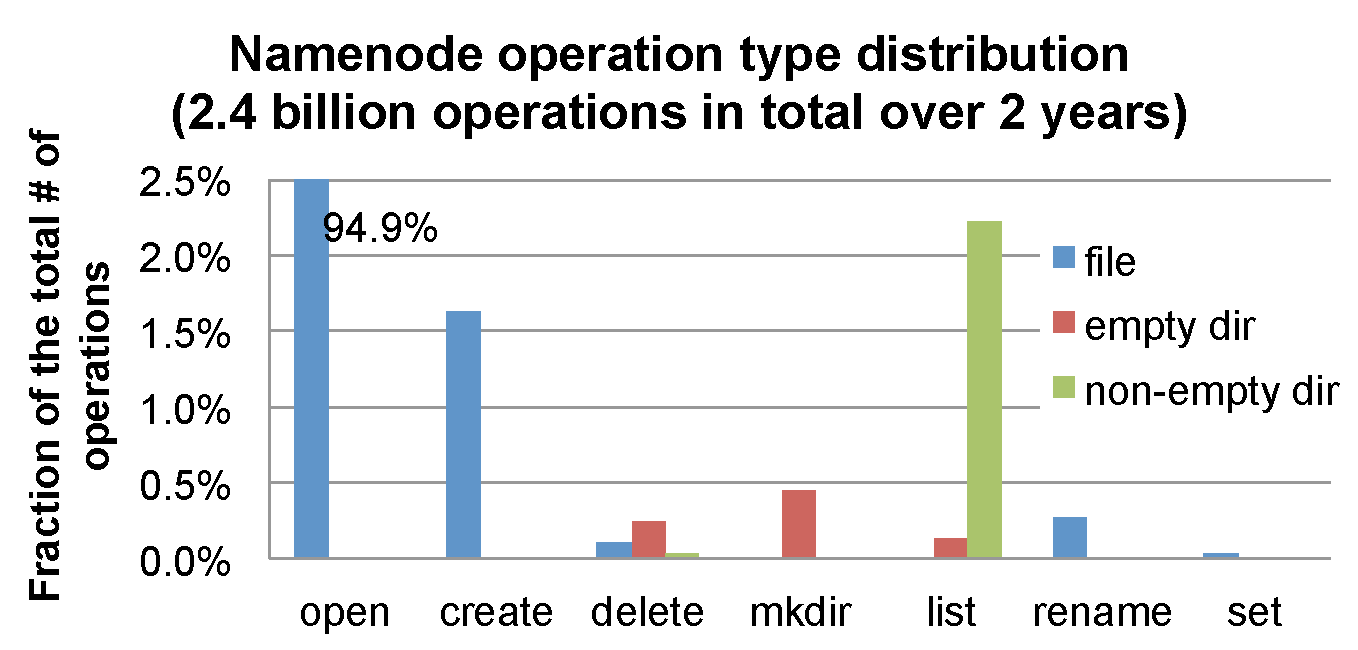
\includegraphics[width=0.55\textwidth]{figs/opdistribution_2}
    }
    \subfigure[Operation depth]{
      \label{fig:opstats:depth}
      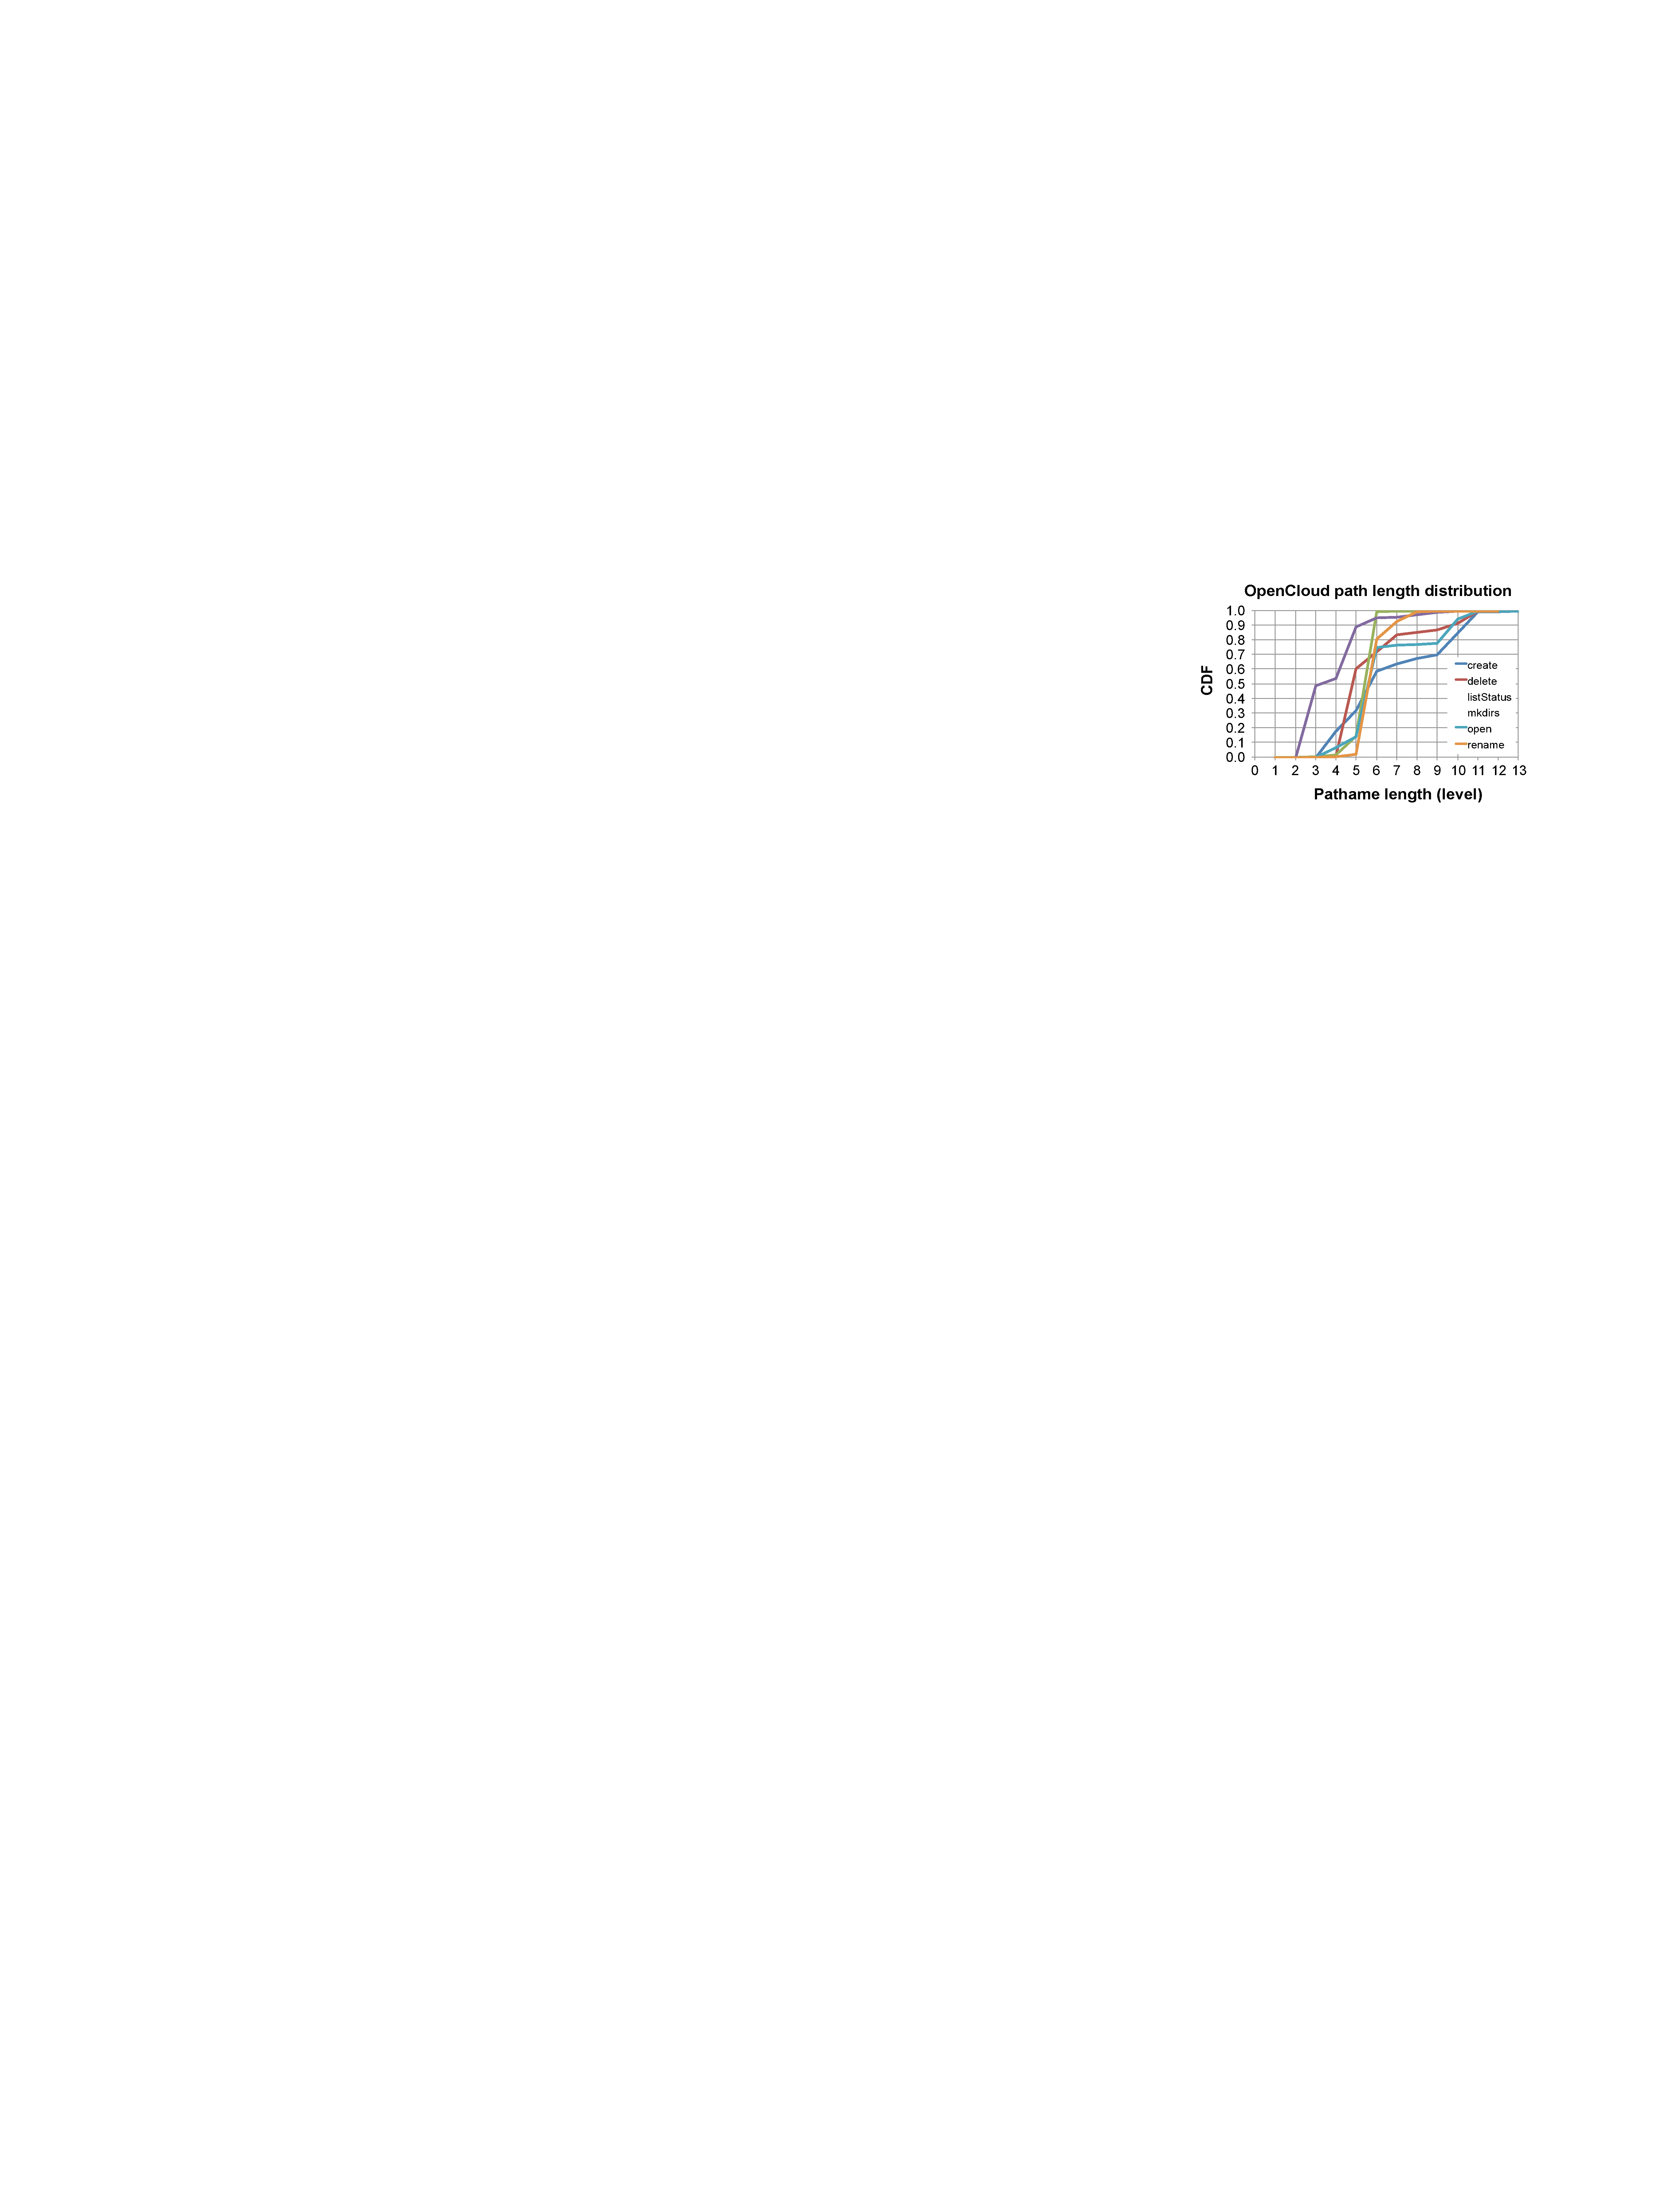
\includegraphics[width=0.35\textwidth]{figs/opdepth}
    }
    \caption{Metadata operation stats in Opencloud}
    \label{fig:opcount_opencloud}
\end{figure*}

As for the static metadata analysis, data was gathered from several clusters from Yahoo!, one cluster in Facebook and OpenCloud at CMU in 2010. With full access to OpenCloud, we have logs of metadata operations since March 2010. Within this period, there are about 94 days of logs missing or incomplete  because of data corruption and log partition full. As shown in figure~\ref{fig:opcount_opencloud}, about $94.86\%$ metadata operations are $open()$ in OpenCloud. Except $open()$, $create()$ and $list()$ are the common operations in the cluster.
